\documentclass[8pt]{beamer}

\usepackage{cmap}
\usepackage[T2A]{fontenc}
\usepackage[utf8]{inputenc}
\usepackage{amsfonts}
\usepackage{amsthm}
\usepackage{mathtools}
\usepackage{color}
\usepackage{hyperref}
\usepackage{graphicx}
\usepackage{pdfpages}
\usepackage{forest}
\usepackage{adjustbox}
\usepackage{times}
\usepackage{tikz}

\mode<presentation>{
    \usetheme{Marburg}
    \usecolortheme{sidebartab}
}

% \newtheorem{theorem}{Theorem}[section]
% \newtheorem{lemma}{Lemma}[section]
% \newtheorem{proposition}{Proposition}[section]
% \newtheorem{corollary}{Corollary}[section]
% \newtheorem{definition}{Definition}[section]
% \newtheorem{remark}{Remark}[section]
% \newtheorem{example}{Example}[section]

\newcommand{\E}{\ensuremath{\mathbb{E}}}
\newcommand{\D}{\ensuremath{\mathbb{D}}}
\renewcommand{\C}{\ensuremath{\mathbb{C}}}
\newcommand{\R}{\ensuremath{\mathbb{R}}}
\newcommand{\Q}{\ensuremath{\mathbb{Q}}}
\newcommand{\Z}{\ensuremath{\mathbb{Z}}}
\renewcommand{\|}{\ensuremath{\hspace{0.1cm} | \hspace{0.1cm}}}

\newcommand{\red}[1]{\textcolor{red}{#1}}
\newcommand{\blue}[1]{\textcolor{blue}{#1}}
\newcommand{\green}[1]{\textcolor{green}{#1}}
\newcommand{\orange}[1]{\textcolor{orange}{#1}}
\newcommand{\teal}[1]{\textcolor{teal}{#1}}
\newcommand{\purple}[1]{\textcolor{purple}{#1}}

\newcommand{\TODO}{\red{TODO}}

\renewcommand{\phi}{\varphi}
\renewcommand{\epsilon}{\varepsilon}
\renewcommand{\le}{\leqslant}
\renewcommand{\ge}{\geqslant}


\begin{document}
    \title[Diffusion Models Testing on Synthetical Data]{Diffusion Models for Time Series\\ Testing on Synthetical Data}
    \author{Fedor Fedorov \& Vanya Vorobiov}
    \date{\today}
    % \institute{Sber}

    \begin{frame}
        \titlepage
    \end{frame}

    \section{Motivation}
    \begin{frame}{Diffusion Models for Time Series: A Fundamental Approach}
        \vspace{-0.3cm}
        \begin{block}{Key Idea}
        \begin{itemize}
            \item Comparative analysis of two diffusion models for time series generation
            \item \textbf{Novel evaluation approach}: Instead of standard industrial datasets, we test on:
            \begin{itemize}
                \item Stochastic processes (e.g., OU process, Gaussian RBF process)
                \item Deterministic functions (where theoretical ground truth is known)
            \end{itemize}
        \end{itemize}
        \end{block}
        
        \vspace{0.2cm}
        \begin{alertblock}{Why This Matters}
        \begin{itemize}
            \item Current literature focuses exclusively on large industrial datasets
            \item Our approach provides:
            \begin{itemize}
                \item Clear theoretical benchmarks
                \item Better understanding of model fundamentals
                \item More meaningful comparison in early-stage research
            \end{itemize}
        \end{itemize}
        \end{alertblock}
        
        \vspace{0.2cm}
        \footnotesize \textit{When the field is in its infancy, controlled experiments on theoretical cases may reveal more than benchmarks on complex real-world data.}
    \end{frame}


    \section{Architecture}
    \subsection{CSDI approach}
    \begin{frame}
            Diffusion key idea~-- model
            \begin{equation}
                p_\theta (x_t|y_{\text{obs}}),
                \label{eq:8}
            \end{equation}
            CSDI arhitecture
            \begin{figure}[h]
                \centering
                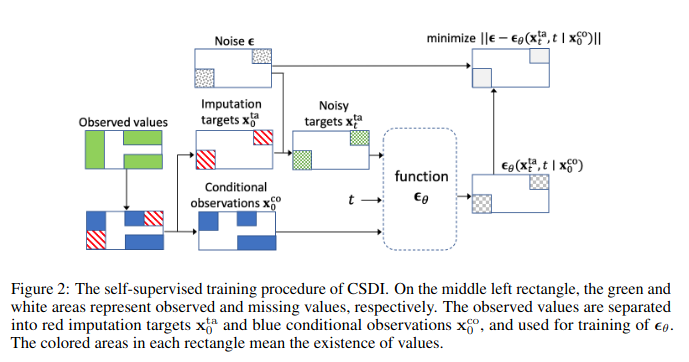
\includegraphics[width=0.8\textwidth]{csdi_architect.png}
            \end{figure}
    \end{frame}

    \subsection{Unconditional approach}
    \begin{frame}
        
            UNCONDITIONAL DIFFUSION KEY IDEA
            
        Let $t \geq 0$ be an arbitrary diffusion step. 
        Applying Bayes' rule, we have
        \begin{equation}
            p_\theta (x_t|y_{\text{obs}}) \propto p_\theta (y_{\text{obs}}|x_t)p_\theta (x_t),
            \label{eq:8}
        \end{equation}
        which yields the following relation between the 
        conditional and marginal score functions,
        \begin{equation}
            \nabla_{x_t} \log p_\theta (x_t|y_{\text{obs}}) = \nabla_{x_t} \log p_\theta (y_{\text{obs}}|x_t) + \nabla_{x_t} \log p_\theta (x_t).
            \label{eq:9}
        \end{equation}

        Given access to the guidance distribution, 
        $p_\theta (y_{\text{obs}}|x_t)$, 
        we can draw samples from $p_\theta (x_t|y_{\text{obs}})$
        \begin{equation}
            p_\theta (x_{t-1}|x_t, y_{\text{obs}}) = \mathcal{N}\left(x_{t-1}; \mu_\theta (x_t, t) + s\sigma^2_t \nabla_{x_t} \log p_\theta (y_{\text{obs}}|x_t), \sigma^2_t I\right).
            \label{eq:10}
        \end{equation}

        $p_\theta (y_{\text{obs}}|x_t)$ modeled as a multivariate Gaussian distribution,
        \begin{equation}
            p_\theta (y_{\text{obs}}|x_t) = \mathcal{N}\left(y_{\text{obs}}|f_\theta (x_t, t), I\right),
        \end{equation}
    \end{frame}

    \section{Tests}
    % ====================== Sine Waves (dim=1) ======================
    \subsection{Sine Waves (1-dimensional)}

    \begin{frame}{Sine Waves (dim=1), Train Size=10,000}
    \begin{block}{Samples}
    \begin{columns}
        \column{0.5\textwidth}
        \centering
        \includegraphics[width=0.9\textwidth]{../test_results/sine_dim_1_train_size_10000/CSDI_sample.png}
        CSDI Sample
        
        \column{0.5\textwidth}
        \centering
        \includegraphics[width=0.9\textwidth]{../test_results/sine_dim_1_train_size_10000/UNCOND_sample.png}
        Unconditional Sample
    \end{columns}
    \end{block}

    \begin{block}{Mean Comparison}
    \centering
    \includegraphics[width=0.6\textwidth]{../test_results/sine_dim_1_train_size_10000/mean.png}
    \end{block}
    \end{frame}

    \begin{frame}{Sine Waves (dim=1), Train Size=50,000}
    \begin{block}{Samples}
    \begin{columns}
        \column{0.5\textwidth}
        \centering
        \includegraphics[width=0.9\textwidth]{../test_results/sine_dim_1_train_size_50000/CSDI_sample.png}
        CSDI Sample
        
        \column{0.5\textwidth}
        \centering
        \includegraphics[width=0.9\textwidth]{../test_results/sine_dim_1_train_size_50000/UNCOND_sample.png}
        Unconditional Sample
    \end{columns}
    \end{block}

    \begin{block}{Mean Comparison}
    \centering
    \includegraphics[width=0.6\textwidth]{../test_results/sine_dim_1_train_size_50000/mean.png}
    \end{block}
    \end{frame}

    \begin{frame}{Sine Waves (dim=1), Train Size=100,000}
    \begin{block}{Samples}
    \begin{columns}
        \column{0.5\textwidth}
        \centering
        \includegraphics[width=0.9\textwidth]{../test_results/sine_dim_1_train_size_100000/CSDI_sample.png}
        CSDI Sample
        
        \column{0.5\textwidth}
        \centering
        \includegraphics[width=0.9\textwidth]{../test_results/sine_dim_1_train_size_100000/UNCOND_sample.png}
        Unconditional Sample
    \end{columns}
    \end{block}

    \begin{block}{Mean Comparison}
    \centering
    \includegraphics[width=0.6\textwidth]{../test_results/sine_dim_1_train_size_100000/mean.png}
    \end{block}
    \end{frame}

    % ====================== Sine Waves (dim=2) ======================
    \subsection{Sine Waves (2-dimensional)}

    \begin{frame}{Sine Waves (dim=2), Train Size=10,000}
    \begin{block}{Samples}
    \begin{columns}
        \column{0.5\textwidth}
        \centering
        \includegraphics[width=0.9\textwidth]{../test_results/sine_dim_2_train_size_10000/CSDI_sample.png}
        CSDI Sample
        
        \column{0.5\textwidth}
        \centering
        \includegraphics[width=0.9\textwidth]{../test_results/sine_dim_2_train_size_10000/UNCOND_sample.png}
        Unconditional Sample
    \end{columns}
    \end{block}

    \begin{block}{Mean Comparison}
    \centering
    \includegraphics[width=0.6\textwidth]{../test_results/sine_dim_2_train_size_10000/mean.png}
    \end{block}
    \end{frame}

    \begin{frame}{Sine Waves (dim=2), Train Size=50,000}
    \begin{block}{Samples}
    \begin{columns}
        \column{0.5\textwidth}
        \centering
        \includegraphics[width=0.9\textwidth]{../test_results/sine_dim_2_train_size_50000/CSDI_sample.png}
        CSDI Sample
        
        \column{0.5\textwidth}
        \centering
        \includegraphics[width=0.9\textwidth]{../test_results/sine_dim_2_train_size_50000/UNCOND_sample.png}
        Unconditional Sample
    \end{columns}
    \end{block}

    \begin{block}{Mean Comparison}
    \centering
    \includegraphics[width=0.6\textwidth]{../test_results/sine_dim_2_train_size_50000/mean.png}
    \end{block}
    \end{frame}

    \begin{frame}{Sine Waves (dim=2), Train Size=100,000}
    \begin{block}{Samples}
    \begin{columns}
        \column{0.5\textwidth}
        \centering
        \includegraphics[width=0.9\textwidth]{../test_results/sine_dim_2_train_size_100000/CSDI_sample.png}
        CSDI Sample
        
        \column{0.5\textwidth}
        \centering
        \includegraphics[width=0.9\textwidth]{../test_results/sine_dim_2_train_size_100000/UNCOND_sample.png}
        Unconditional Sample
    \end{columns}
    \end{block}

    \begin{block}{Mean Comparison}
    \centering
    \includegraphics[width=0.6\textwidth]{../test_results/sine_dim_2_train_size_100000/mean.png}
    \end{block}
    \end{frame}

    % ====================== OU (dim=1) ======================
    \subsection{Ornstein-Uhlenbeck (1-dimensional)}
    \begin{frame}{Ornstein-Uhlenbeck (dim=1)}
        \begin{block}{Samples}
        \begin{columns}
            \column{0.5\textwidth}
            \centering
            \includegraphics[width=0.9\textwidth]{../test_results/ou1dcsdi.jpg}
            CSDI Sample
            
            \column{0.5\textwidth}
            \centering
            \includegraphics[width=0.9\textwidth]{../test_results/ou1duncond.jpg}
            Unconditional Sample
        \end{columns}
        \end{block}
    
    \end{frame}

    % ====================== OU (dim=2) ======================
    \subsection{Ornstein-Uhlenbeck (2-dimensional)}
    \begin{frame}{Ornstein-Uhlenbeck (dim=2)}
        \begin{block}{Samples}
        \begin{columns}
            \column{0.5\textwidth}
            \centering
            \includegraphics[width=0.9\textwidth]{../test_results/ou2dcsdi.jpg}
            CSDI Sample
            
            \column{0.5\textwidth}
            \centering
            \includegraphics[width=0.9\textwidth]{../test_results/ou2duncond.jpg}
            Unconditional Sample
        \end{columns}
        \end{block}
    
    \end{frame}

    % ====================== Gaussian Process (dim=1) ======================
    \subsection{Gaussian Process (1-dimensional)}

    \begin{frame}{Gaussian Process (dim=1), Train Size=10,000}
    \begin{block}{Samples}
    \begin{columns}
        \column{0.5\textwidth}
        \centering
        \includegraphics[width=0.9\textwidth]{../test_results/gp_dim_1_train_size_10000/CSDI_sample.png}
        CSDI Sample
        
        \column{0.5\textwidth}
        \centering
        \includegraphics[width=0.9\textwidth]{../test_results/gp_dim_1_train_size_10000/UNCOND_sample.png}
        Unconditional Sample
    \end{columns}
    \end{block}

    \begin{block}{Mean Comparison}
    \centering
    \includegraphics[width=0.6\textwidth]{../test_results/gp_dim_1_train_size_10000/mean.png}
    \end{block}
    \end{frame}

    \begin{frame}{Gaussian Process (dim=1), Train Size=25,000}
    \begin{block}{Samples}
    \begin{columns}
        \column{0.5\textwidth}
        \centering
        \includegraphics[width=0.9\textwidth]{../test_results/gp_dim_1_train_size_25000/CSDI_sample.png}
        CSDI Sample
        
        \column{0.5\textwidth}
        \centering
        \includegraphics[width=0.9\textwidth]{../test_results/gp_dim_1_train_size_25000/UNCOND_sample.png}
        Unconditional Sample
    \end{columns}
    \end{block}

    \begin{block}{Mean Comparison}
    \centering
    \includegraphics[width=0.6\textwidth]{../test_results/gp_dim_1_train_size_25000/mean.png}
    \end{block}
    \end{frame}

    \begin{frame}{Gaussian Process (dim=1), Train Size=50,000}
    \begin{block}{Samples}
    \begin{columns}
        \column{0.5\textwidth}
        \centering
        \includegraphics[width=0.9\textwidth]{../test_results/gp_dim_1_train_size_50000/CSDI_sample.png}
        CSDI Sample
        
        \column{0.5\textwidth}
        \centering
        \includegraphics[width=0.9\textwidth]{../test_results/gp_dim_1_train_size_50000/UNCOND_sample.png}
        Unconditional Sample
    \end{columns}
    \end{block}

    \begin{block}{Mean Comparison}
    \centering
    \includegraphics[width=0.6\textwidth]{../test_results/gp_dim_1_train_size_50000/mean.png}
    \end{block}
    \end{frame}

    % ====================== Gaussian Process (dim=2) ======================
    \subsection{Gaussian Process (2-dimensional)}

    \begin{frame}{Gaussian Process (dim=2), Train Size=5,000}
    \begin{block}{Samples}
    \begin{columns}
        \column{0.5\textwidth}
        \centering
        \includegraphics[width=0.9\textwidth]{../test_results/gp_dim_2_train_size_5000/CSDI_sample.png}
        CSDI Sample
        
        \column{0.5\textwidth}
        \centering
        \includegraphics[width=0.9\textwidth]{../test_results/gp_dim_2_train_size_5000/UNCOND_sample.png}
        Unconditional Sample
    \end{columns}
    \end{block}

    \begin{block}{Mean Comparison}
    \centering
    \includegraphics[width=0.6\textwidth]{../test_results/gp_dim_2_train_size_5000/mean.png}
    \end{block}
    \end{frame}

    \begin{frame}{Gaussian Process (dim=2), Train Size=10,000}
    \begin{block}{Samples}
    \begin{columns}
        \column{0.5\textwidth}
        \centering
        \includegraphics[width=0.9\textwidth]{../test_results/gp_dim_2_train_size_10000/CSDI_sample.png}
        CSDI Sample
        
        \column{0.5\textwidth}
        \centering
        \includegraphics[width=0.9\textwidth]{../test_results/gp_dim_2_train_size_10000/UNCOND_sample.png}
        Unconditional Sample
    \end{columns}
    \end{block}

    \begin{block}{Mean Comparison}
    \centering
    \includegraphics[width=0.6\textwidth]{../test_results/gp_dim_2_train_size_10000/mean.png}
    \end{block}
    \end{frame}

    \begin{frame}{Gaussian Process (dim=2), Train Size=20,000}
    \begin{block}{Samples}
    \begin{columns}
        \column{0.5\textwidth}
        \centering
        \includegraphics[width=0.9\textwidth]{../test_results/gp_dim_2_train_size_20000/CSDI_sample.png}
        CSDI Sample
        
        \column{0.5\textwidth}
        \centering
        \includegraphics[width=0.9\textwidth]{../test_results/gp_dim_2_train_size_20000/UNCOND_sample.png}
        Unconditional Sample
    \end{columns}
    \end{block}

    \begin{block}{Mean Comparison}
    \centering
    \includegraphics[width=0.6\textwidth]{../test_results/gp_dim_2_train_size_20000/mean.png}
    \end{block}
    \end{frame}

    \section{Key Findings \& Future Directions}
    \begin{frame}{Conclusions and Next Steps}

        \begin{block}{Key Takeaways}
        \begin{itemize}
            \item Our tests reveal that current diffusion models often struggle with basic synthetic tasks
            \item Performance varies significantly between different architectures
            \item Simple test cases expose limitations not visible in complex real-world benchmarks
        \end{itemize}
        \end{block}
        
        \vspace{0.4cm}
        
        \begin{alertblock}{Future Work}
        \begin{itemize}
            \item Explore additional model architectures
            \item Conduct more comprehensive testing
            \item Develop better evaluation approaches for fundamental properties
        \end{itemize}
        \end{alertblock}
        
    \end{frame}

    

    \section{Bibliography}
\begin{frame}{Bibliography}
    \begin{thebibliography}{99}
        \bibitem{yuan2024diffusionts} 
        Xinyu Yuan and Yan Qiao, 
        \textit{Diffusion-TS: Interpretable Diffusion for General Time Series Generation}, 
        The Twelfth International Conference on Learning Representations, 2024.
        
        \bibitem{tashiro2021csdi} 
        Yusuke Tashiro, Jiaming Song, Yang Song and Stefano Ermon, 
        \textit{CSDI: Conditional Score-based Diffusion Models for Probabilistic Time Series Imputation}, 
        Advances in Neural Information Processing Systems, 2021.
    \end{thebibliography}
\end{frame}
\end{document}
